\chapter{Discussion and Future Work}
\label{chap:discussion-future}

The evaluation of the integrated system demonstrates that combining probabilistic
forecasting with hierarchical \ac{RCA} yields actionable, economically interpretable
anomaly management at portfolio scale. At the same time, the transition from a
controlled synthetic benchmark to heterogeneous industrial deployments exposes
limitations in contextual observability, baseline health assumptions, and the
expressiveness of sequential foundation models. This chapter reflects critically on
these gaps and outlines concrete directions for strengthening methodological coverage
and operational robustness.

\section{Critical Reflection on System Design}

The current \ac{RCA} implementation localizes anomalies primarily through signed
financial attribution across sub-meters (Section~\ref{sec:root-cause-analysis}).
This is effective for answering \emph{where} excess consumption accumulates and
supports \textbf{O\ref{obj:hierarchical-diagnosability}} and
\textbf{O\ref{obj:economic-interpretability}}, but it provides limited insight into
\emph{why} the deviation occurred within the control layer
(Foundations Section~\ref{sec:building-energy-data} / causal chain discussion in
Section~\ref{subsec:causal-chain-energy-consumption}). In many facilities, the same consumption pattern can arise
from distinct causes (e.g., manual override, schedule misconfiguration, actuator
fault). Future iterations should therefore extend diagnostics beyond metering
attribution by incorporating \emph{operational state signals} for major consumers
(e.g., valve positions, fan speeds, compressor staging, setpoints). This would enable
causal consistency checks such as: ``is the spike explained by a corresponding change
in control demand?'' and would strengthen context-aware interpretation
(\textbf{O\ref{obj:contextual-fidelity}}) while improving the explainability of
high-impact events.

A second design boundary is the \emph{scope of anomaly classes}. The proposed framework
is strong at detecting deviations in consumption relative to context-conditioned
baselines, but it may not
detect \emph{logic conflicts that are consistently present in the baseline}, such as
simultaneous heating and cooling, chronic simultaneous reheat, or persistent
inefficiencies that have become ``normal'' operation. This is not a modelling failure
but a baseline-definition limitation and directly relates to
\textbf{O\ref{obj:persistence-preservation}}.

\section{Robust Baseline Health Without Manual User Selection}
\label{sec:baseline-health-future}

The current production assumption is that historical data preceding activation is
sufficiently healthy for establishing a normative reference. In real buildings this
is frequently violated: persistent faults may exist for months, and ``normal'' may
already include inefficiency (Foundations Sections~\ref{subsec:temporal-autocorrelation-persistence}
and~\ref{subsec:statistical-distribution-stochastic-noise} on non-stationarity and
persistence; Section~\ref{sec:critique-sequential} on contamination effects). A manual
``gold-standard baseline'' UI would shift responsibility to the operator and does not
scale across tenants, contradicting the deployment objective
\textbf{O\ref{obj:horizontal-scalability}}.

A more robust direction is to integrate \emph{classical rule-based energy baselining
and detection} as a complementary layer, as discussed in
Section~\ref{sec:classical-energy-anomaly-detection}. Rule-based checks (e.g., schedule
violations, simultaneous heating/cooling, minimum runtime constraints, holiday/weekend
rules) can be used in two ways:

\begin{enumerate}
    \item \textbf{Baseline screening:} automatically tag historical intervals as
    ``likely healthy'' vs.\ ``likely faulty'' and preferentially sample healthy
    segments for the model context. This reduces the risk that persistent faults are
    learned as normal and strengthens \textbf{O\ref{obj:persistence-preservation}} and
    \textbf{O\ref{obj:contextual-fidelity}} without requiring user intervention.

    \item \textbf{Coverage expansion:} detect fault classes that are not consumption
    outliers but are operational contradictions (e.g., heating and cooling overlap)
    even if they were present in the baseline. This provides robustness against
    unhealthy historical data and complements the probabilistic deviation detector.
\end{enumerate}

Operationally, this hybrid approach would yield a more complete anomaly portfolio:
probabilistic scoring for contextual deviations (weather/occupancy adjusted) and
deterministic rules for control-logic violations and persistent inefficiencies. The
combination directly addresses the failure mode described in
Section~\ref{sec:critique-sequential} (adaptation and contamination) and improves
diagnostic depth beyond pure metering attribution.

\section{Context and Modality Expansion}

The current implementation focuses on electricity meters enriched with meteorological
covariates. A natural extension is to generalize the same pipeline to additional
utilities (e.g., gas, water, thermal energy, and emissions-related signals), thereby
broadening applicability while preserving the same methodological objectives of
context-conditioned baselines and signed impact quantification
(\textbf{O\ref{obj:contextual-fidelity}}, \textbf{O\ref{obj:economic-interpretability}}).

\section{Future Architecture: Universal Energy Feature Forecaster}
\label{sec:universal-feature-forecaster}

Chronos-2 was selected for deployment due to its operational scalability and robust
quantile outputs (Section~\ref{sec:model-selection-rationale}), but the implementation
also exposes structural limitations of sequential time-series foundation models:

\begin{itemize}
    \item \textbf{Sequence constraint:} inference requires temporally contiguous
    context immediately preceding the forecast timestamp, limiting the ability to use
    non-contiguous ``healthy'' reference segments (Section~\ref{sec:baseline-health-future}).

    \item \textbf{Autoregressive sensitivity:} sequential dependence can amplify
    short-term autocorrelation and induce adaptation effects (Section~\ref{sec:critique-sequential}),
    requiring mitigation logic in production.

    \item \textbf{Limited distribution access:} forecasts are primarily consumed as
    quantile bounds, which enables calibrated envelopes but does not expose an
    explicit multimodal density comparable to \acp{MDN} (Sections~\ref{subsec:mdn-solution}
    and~\ref{sec:md-anomaly-scoring}).
\end{itemize}

A forward-looking direction is a specialized foundation model designed explicitly as a
\emph{universal energy feature forecaster}. Instead of next-step sequence prediction,
the model would perform conditional regression from \emph{context features} to a target
distribution:
\[
p(y \mid \mathbf{x}, \mathcal{B}),
\]
where $\mathbf{x}$ are covariates (weather, calendar, occupancy proxies, operational
state) and $\mathcal{B}$ is an in-context baseline set of feature--target examples.
Critically, $\mathcal{B}$ would not need to be temporally contiguous or adjacent to
the forecast time; it could be composed from automatically screened healthy segments
across the year (Section~\ref{sec:baseline-health-future}). This directly targets
\textbf{O\ref{obj:contextual-fidelity}}, \textbf{O\ref{obj:drift-robustness}}, and
\textbf{O\ref{obj:persistence-preservation}} by decoupling the normative reference
from immediate sequential inputs.

\subsection{Mixture-Distribution Output and Distribution-Aware Scoring}

To recover the expressiveness of mixture modelling without per-meter training, the
model should output an explicit multimodal density (e.g., token-mixture or continuous
mixture parameters). This would enable likelihood-based and \ac{DQ}-based anomaly
scoring (Section~\ref{sec:md-anomaly-scoring}) with time-comparable severity scaling,
while keeping the zero-shot generalization benefits emphasized in
Section~\ref{sec:model-selection-rationale}. In effect, this would combine the
portfolio robustness of \acp{TSFM} with the distributional fidelity of \acp{MDN},
strengthening \textbf{O\ref{obj:distributional-validity}} without the instability and
coverage gaps observed in trainable mixture architectures.

\subsection{Decision Support and IPMVP-Style Verification}

A feature-conditional, baseline-set forecaster also enables systematic baseline
comparison without retraining: the same operating point (same covariates $\mathbf{x}$)
can be evaluated under multiple baseline contexts $\mathcal{B}_1,\mathcal{B}_2$ to
quantify the expected change attributable to interventions. This naturally aligns with
Measurement and Verification practices such as the \ac{IPMVP}: predicted counterfactual consumption
under a pre-intervention baseline can be compared against a post-intervention baseline
to estimate savings under matched conditions. This extends the system beyond fault
detection into continuous efficiency verification, directly reinforcing the economic
motivation of Chapter~\ref{chap:introduction} and strengthening
\textbf{O\ref{obj:economic-interpretability}} at portfolio scale.
Figure~\ref{fig:ipmvp-overview} summarizes the \ac{IPMVP} comparison workflow that underpins
these verification steps~\parencite{ipmvp-protocol}.

\begin{figure}[H]
\centering
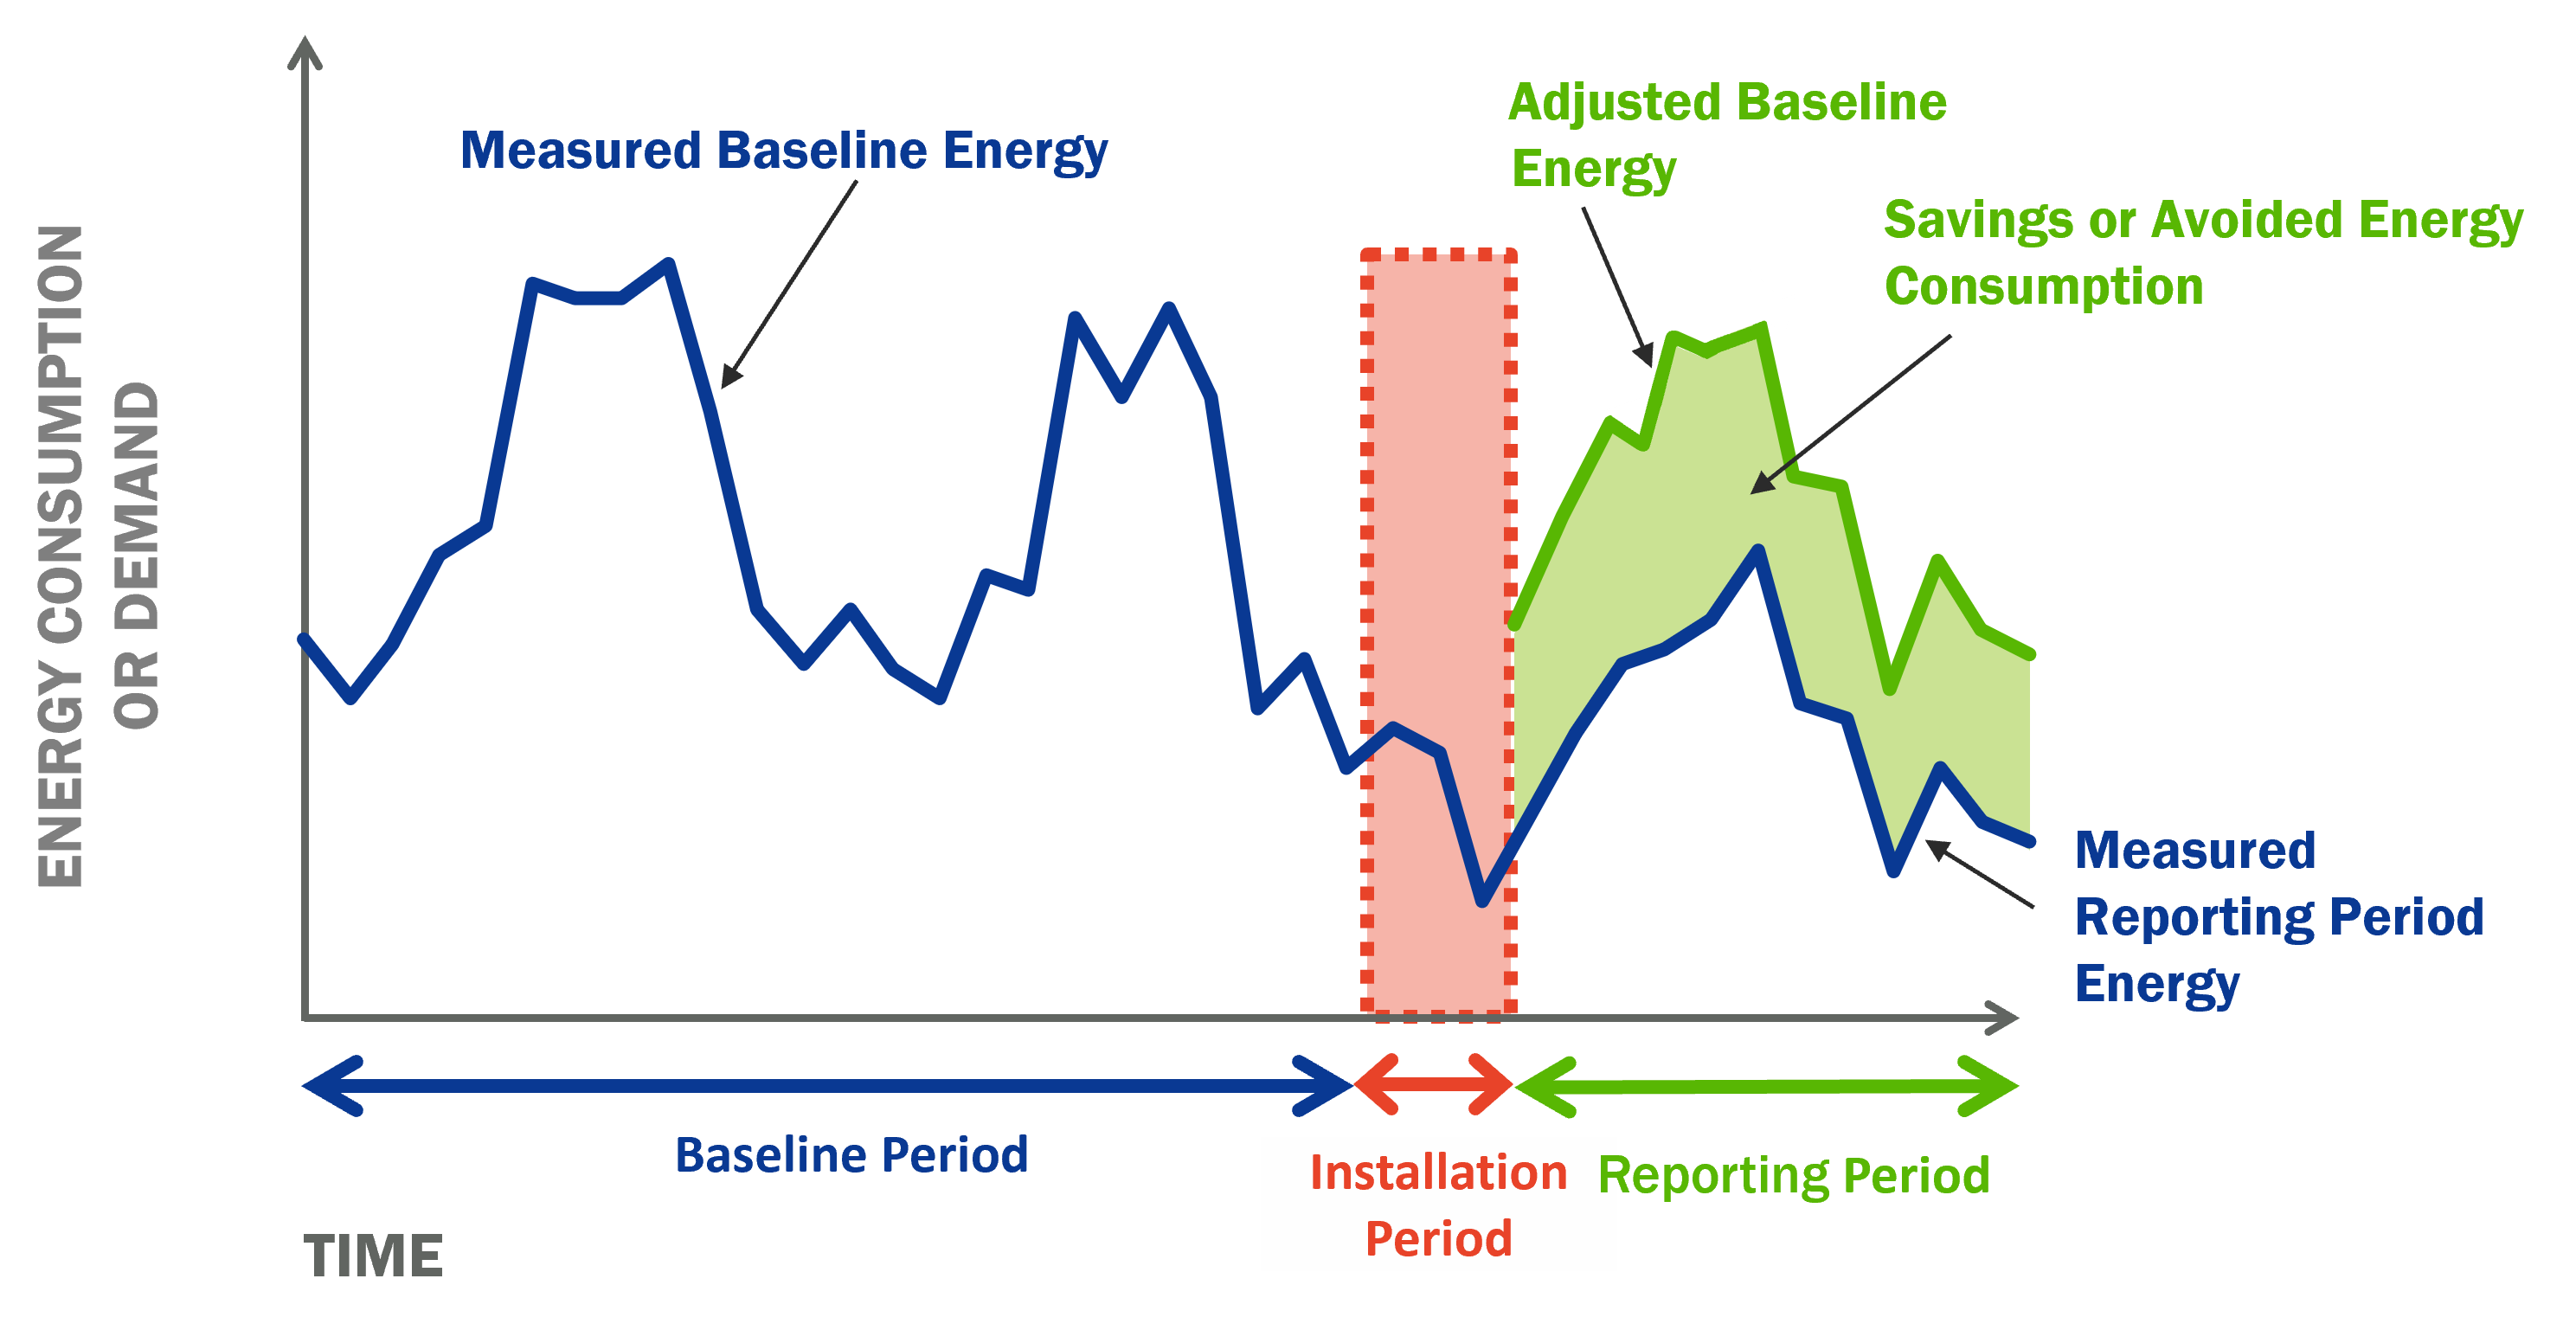
\includegraphics[width=0.85\textwidth]{images/IPMVP.png}
\caption{\ac{IPMVP} verification workflow across baseline and reporting periods, adapted from \textcite{ipmvp-protocol}.}
\label{fig:ipmvp-overview}
\end{figure}

